\chapter{Conclusion and Future Work}
\label{CAFW}

\section{Conclusion}
\label{Conclusion}
Understanding the relationship that phages have with bacteria and the environment is complex. 
Even for a $1\times1\times1$ system, the system is already complex. 
Not including $M$ and the initial infected bacteria population, the parameter input space is 12 dimensions large. 
Although quite small in comparison to other larger models, analyzing 12 unique parameters and their interactions takes effort. 
Finding parameter values that result in quality graphs is not the easiest task, although knowing the expected values and the biological relevance makes the task easier. 
Finding a set of parameters that results in behavior that is worth analyzing takes time. 
Using interactive graphs like what I created helps the user to look through the parameter space to find interesting behavior and gain a deeper understanding of the model. 
However even a simple change in the parameter input like in \Cref{fig:created:initial_value_analysis_UB_50_500_a_good_plot} vs \Cref{fig:created:initial_value_analysis_UB_50_500_a_good_plot_2} shows vastly contrasting behavior, despite both graphs being realistic. 

Trying to expand an analysis into a $p\times b\times r$ system becomes even more complicated due to the interconnected nature of the entities. 
With larger and larger systems small changes in a single parameter will not have big of an influence on the final output. 
But if the parameter value does have an influence, it has a cascading effect on the whole network. 
Increasing the infection rate of phage 1 will slow the growth of the bacteria 1. 
With slower bacteria 1 growth, phage 2 is affected as there are less bacteria 1 to infect (assuming that phage 2 can infect bacteria 1). With lower phage 2 count, bacteria 2 can grow, using more resources. 
The 


And how do you change the parameter value of the vector or matrix representation? 
If you want to chnage $\tau$ to $1.5$, how do you do that? 
Do you only change one value in the vector or matrix, so for example $\tau = \begin{bmatrix} 1.43 & 0.98 & 1.13\end{bmatrix}$ becomes $\tau = \begin{bmatrix} 1.5 & 0.98 & 1.13\end{bmatrix}$? 
Do you set each value in the vector or matrix the same, so $\tau = \begin{bmatrix} 1.43 & 0.98 & 1.13\end{bmatrix}$ becomes $\tau = \begin{bmatrix} 1.5 & 1.5 & 1.5\end{bmatrix}$? 
Do you respect the different values in the vector or matrix by shifting the values from the average value? 
So $\tau = \begin{bmatrix} 1.43 & 0.98 & 1.13\end{bmatrix}$ becomes $\tau = 1.5 - \frac{1.43 + 0.98 + 1.13}{3} = 1.5-1.18 = 0.32 = \begin{bmatrix} 1.43+0.32 & 0.98+0.32 & 1.13+0.32\end{bmatrix} = \begin{bmatrix} 1.75 & 1.3 & 1.45\end{bmatrix}$. 
How does that change if there is $NaN$? 
Do you treat it as 0? 
Do you skip it and dont let that value count towards the average value to shift the vector and matrix values by. 

\section{Future Work}
\label{Future Work}
Next steps would be to give the model to the lab technicians running lab experiments so that they can verify the results as seen in the output by comparing the lab results with the model output. 
With the lab results, the model can be adapted to better fit the lab results. 
This can be done by changing parameter values, or by changing the model equation. 
The user can decide to add the Monod microbial growth model to the growth of the bacteria, or adapt the Monod equation to being dependent on multiple sources. 
Using the model, the technicians can improve and validate their methods. 
If the empirical results significantly deviate from the model results, the technician can review to see if their method is appropriate and follows protocol. 
They might have accidentally not added enough resources, or accidentally miscalculated the initial concentration of bacteria. 

\subsection{Other Models}
There are numerous considerations to account for when modelling phages and bacteria, with numerous ways to go about the considerations. 
Each model has its pros and cons. 
Take the exponential population growth model 
\begin{align}
    \frac{dP}{dt} &= rP \\
    P(t) &= P_0e^{rt} 
\end{align}
where $P(t)$ is the population at time $t$, $P_0$ is the initial population, and $r$ is the growth rate. 
This model acts as a nice introduction to population modelling. It can accurately fit the exponential growth bacteria experience in a petri dish. 
However, this basic model does not account for a spatial and resource consumption. 
Eventually the bacteria run out of space and resources, and start to die out. 
A population can not grow exponentially forever, the resources can only support a maximum population, the carrying capacity. 
The model can be adapted to include a carrying capacity (the max population level that can be reached), where the new updated model is 
\begin{align}
    \frac{dP}{dt} &= rP(1-\frac{P}{K}) \\ 
    P &= \frac{K}{1 + (\frac{K-N_0}{N_0})e^{-rt}}
\end{align}
where $K$ is the carrying capacity. This adapted model, the logistic growth model better accounts for the eventual restriction of population growth. 

\Cref{fig:created:exponential_vs_logistic_growth} shows how the carrying capacity has a large influence on the speed and growth trajectory of a population. 
The logistic curve initially follows the exponential curve before the maximum growth rate is reached and starts to slow down and taper off as the population asymptotically approaches the carrying capacity $K=200$. 

\begin{figure}
    \centering
    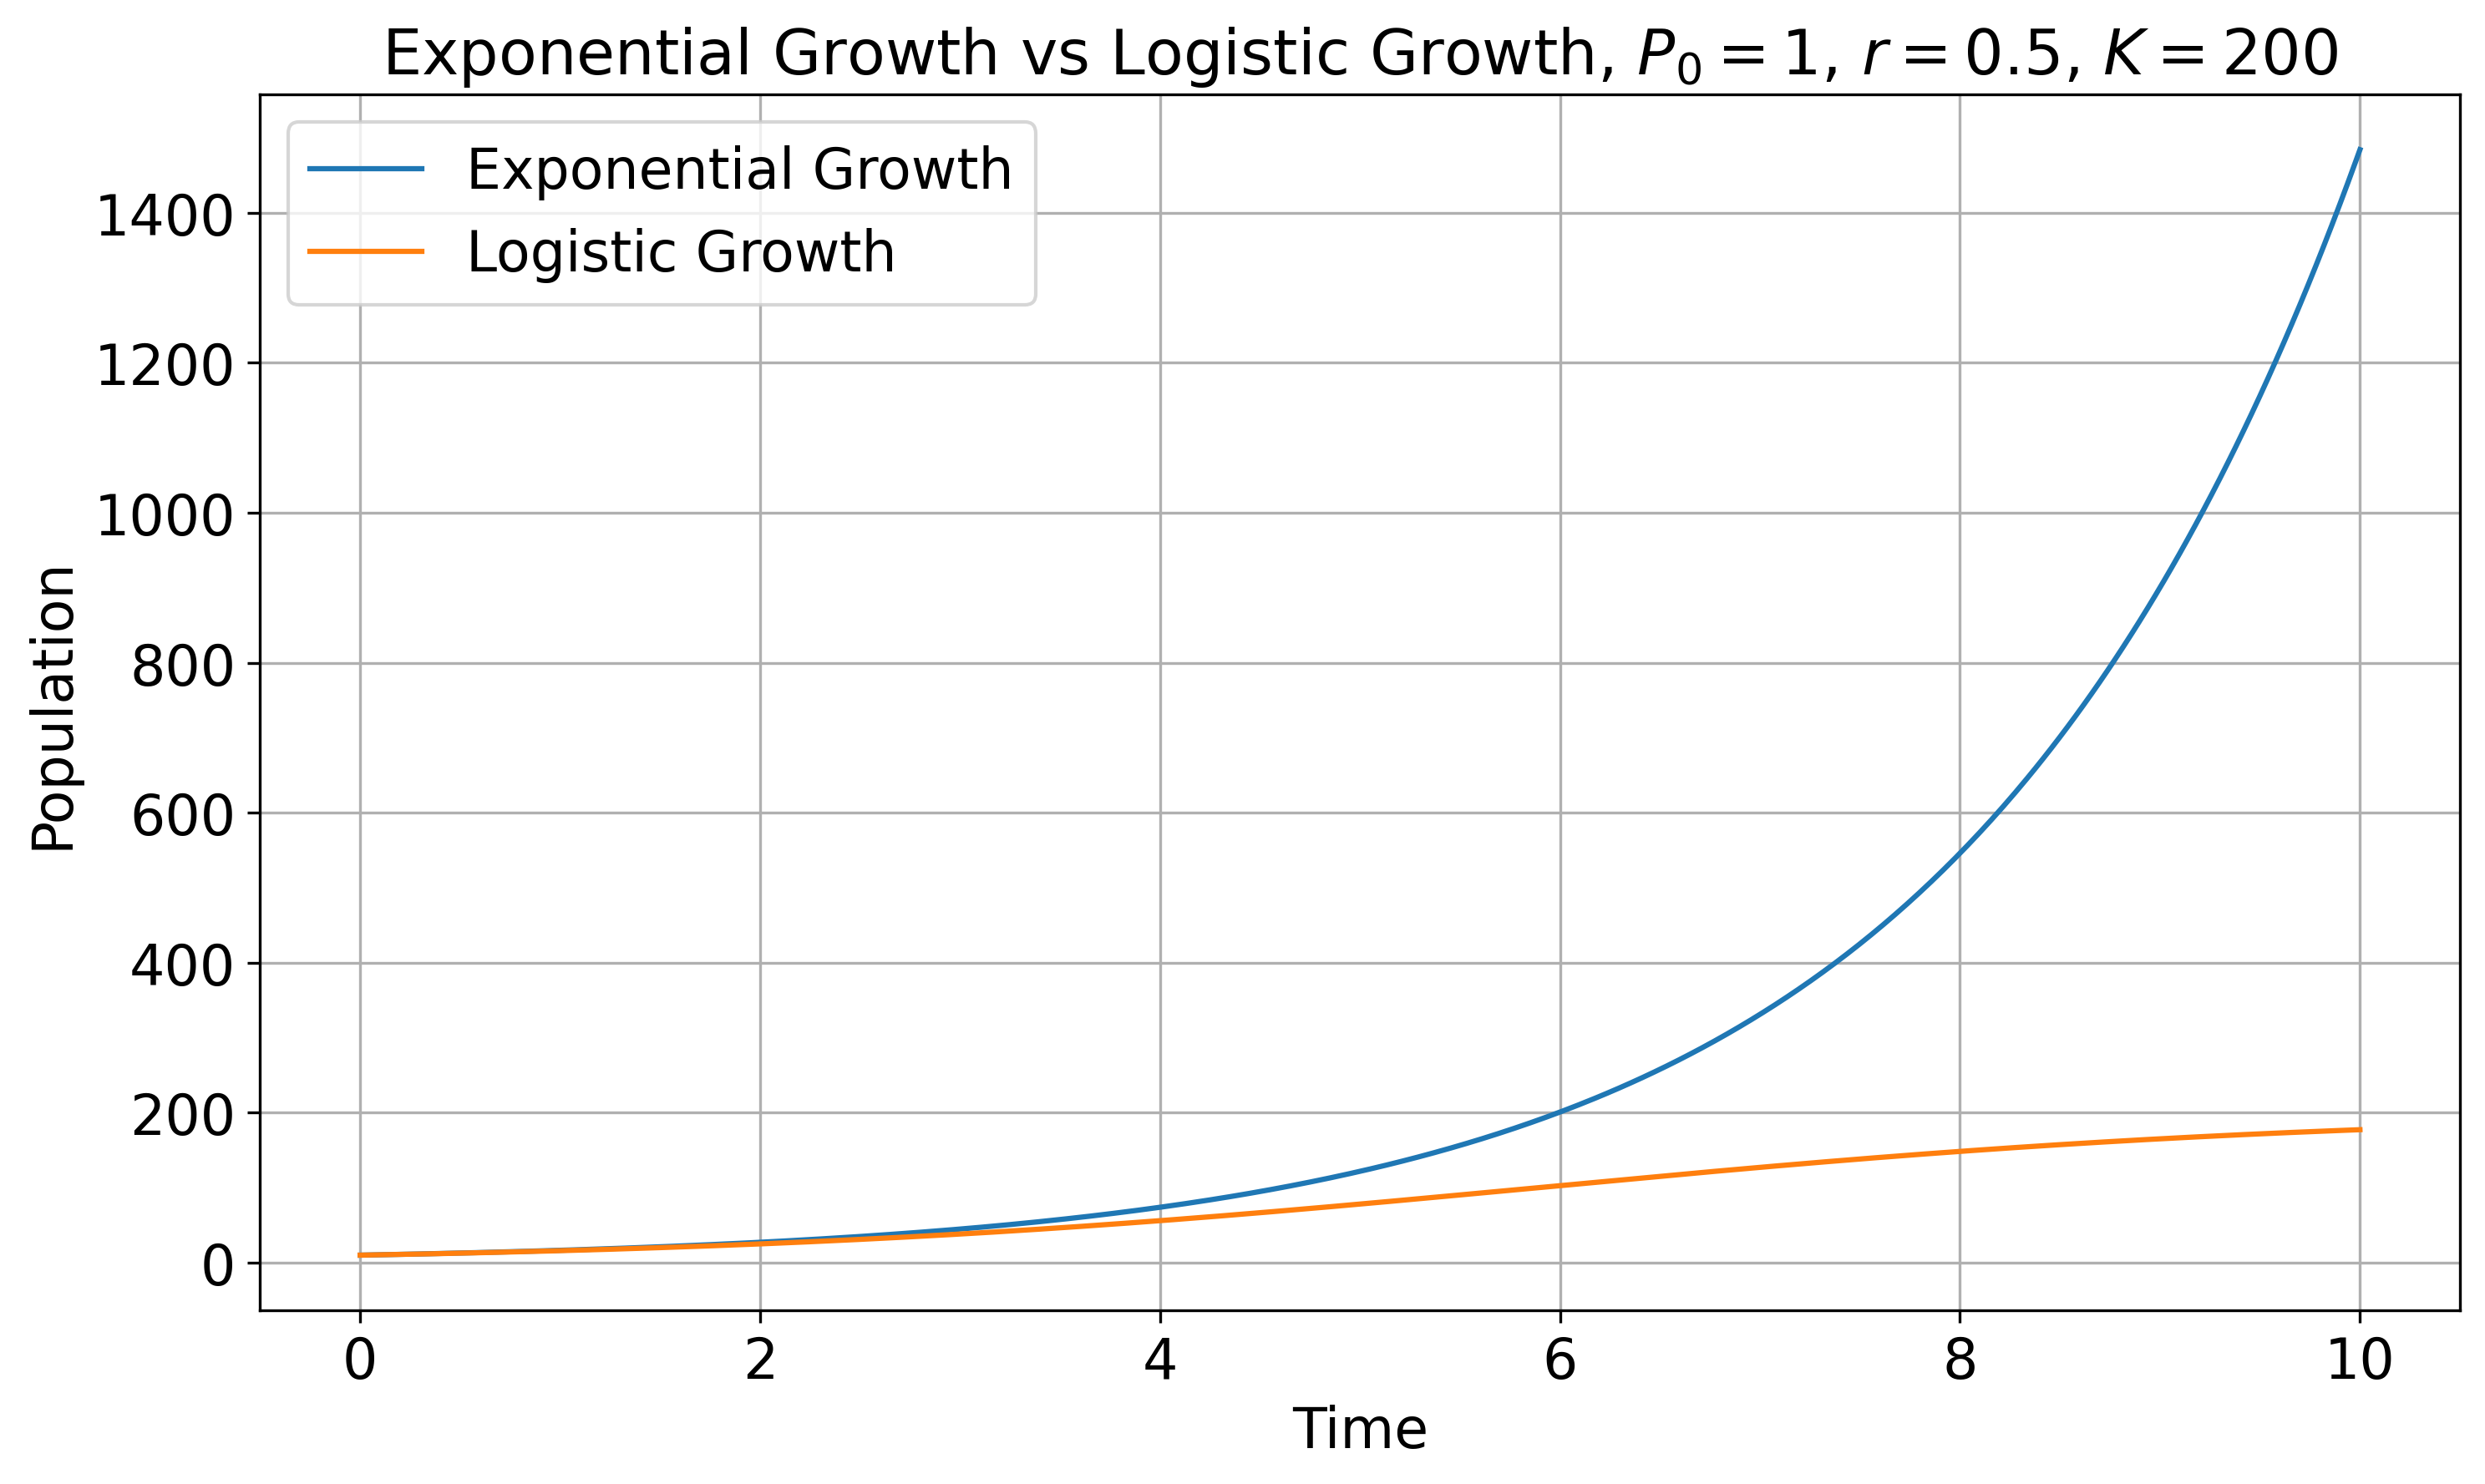
\includegraphics[width=0.5\linewidth]{Plots/Created/exponential_vs_logistic_growth.png}
    \caption{Exponential growth curve vs logistic growth}
    \label{fig:created:exponential_vs_logistic_growth}
\end{figure}

A further step would be to introduce competition between other bacteria. 
For example, a $p_{0, 1}\cdot P_0 \cdot P_1$ term can be subtracted from the logistic growth curve. 
This term accounts for competition between Populace 0 and Populace 1, with $p_{0, 1}$ being the interaction factor between $P_0$ and $P_1$. 
Assuming $P_0$ is being looked at and $P_0$ has a high value, if $P_1$ is high, then a lot of $P_0$ is going to die out due to the competition with $P_1$. 
If $P_1$ has a low population, then not many $P_0$ are going to die out due to less competition with $P_1$. \\ 

The model can be further extended by accounting for temperature, pH, more interactions between other entities, the constant addition and removal of other entities, and other considerations. 

\subsubsection{Model Replication}
Peer review is very important in research. 
So being able to replicate other models like that of \citet{nilssonCocktailComputerProgram2022} is another way to further extend this research. 
A benefit of implementing Cocktail's model is that it would be possible to model multiple bacteria and phages at the same time, as noted as a limitation in \Cref{sec:literature:cocktail_and_phagedyn_limitations}. 
The model can also be adapted by introducing new environmental factors like pH or UV. 
Cocktail supports adding more phages at set times, but only at most three times. 
The model can be extended by allowing more times when phages can be added. 

\subsubsection{Debris}
Looking further into the debris and its effects would be a next step in the project. 
It was casually shown how adding a debris term increased the survivability of the bacteria populations, with showing on average a higher uninfected bacteria population, and lower uninfected and phage population count. 


\subsubsection{Spatial simulations}
https://www.sciencedirect.com/science/article/abs/pii/S0022519318305368
The ODE models work very nicely when there is no consideration for space and 2D/3D-space dimensionality. 
Spatial models complicate the simulation, making it harder to analyze. 
Data collection and analysis becomes harder. 
Unique and novel analysis and visualization methods have to be created to be able to represent and visualize the data through space and time. 
\paragraph{PDE}
PDE can be used to add space to an ODE model. 
The general formula, as given by 
\[
    \frac{\partial u}{\partial t} = D\nabla^2u + f(u, x, y, \dots, t)
\] where $u(x, y, \dots, t)$ is the population density of interest, $D$ is the diffusion constant, $\nabla^2$ is the derivative of each spatial direction, and $f(x, y, \dots, t)$ is the function encapsulating growth, death, and interactions dynamics. 
Modelling the localization of phages on a petri dish would be of interest. 

\subparagraph{Discretization}
The dimensions can be discretized into boxes of dimensions $\delta x, \delta y, \dots$. 
This transforms the PDE into a system of difference equations, which can be solved numerically. 
For example, the Laplacian term $\nabla^2 u$ in 2D can be approximated using finite differences as:
\[
    \nabla^2 u \approx \frac{u_{i+1,j} - 2u_{i,j} + u_{i-1,j}}{\delta x^2} + \frac{u_{i,j+1} - 2u_{i,j} + u_{i,j-1}}{\delta y^2}
\]
where $u_{i,j}$ represents the value of $u$ at the grid point $(i, j)$. 
This discretization allows the PDE to be solved iteratively over a grid, enabling spatial simulations of population dynamics. 
Each box can be represented by a matrix, and the population value can be displayed as a heatmap using visualization software. 

\subsection{Lab Work}
A next logical step would be to complete lab work to obtain curves that could be used to compare the simulation results with the lab results. 
If the curves are significantly different from that of the ODE model, a new ODE model can be created. 
Curve fitting algorithms can be used to numerically find the interaction parameters for the new ODE model. 
Using the simulation software would save time, money, and resources as fewer experiments would have to be run. 

The lab work would act as an important model validation step. 
\citet{deyEmergentHigherorderInteractions2025} showed how their ODE model would eventually diverge from the lab-produced ODE curve. 
They were able to achieve a better curve fit by adapting the model to include the debris term. 

Future lab work can also include finding out which bacteria, phages, and resources are found in marine water via samples taken from the environment. 
The next step would be to build an interaction network, along with experimentally finding out the interaction parameter values using experimental lab work. 
Researchers can predict how the system would behave under new untested conditions, saving money and time. 
It might also tell researchers if they made a mistake during testing. 
If the model says the system should behave in one way, but the system acts differently, the researcher can review their methods and maybe make changes to how they run the experiments. 
All in all, having a model that takes seconds to run will help aid researchers better understand the system. 

\subsubsection{Environmental Modelling}
Many results in research papers come from controlled lab settings. 
As a next step, researchers can actively collect daily water samples and measure phage, bacteria, and resource concentrations. 
Collecting samples for over a year would create an ODE-like population curve of the entities. 
This approach would provide deeper insights into the dynamics of bacteria and phage populations in natural environments, at the loss of control over conditions. 
By continuously monitoring environmental factors such as hourly temperature, rainfall, and the concentrations of each entity, researchers can gain a deeper understanding of the causal relationships within the ecosystem.
By conducting the experiment over the course of a year, short-term fluctuations in daily measurements are averaged out, resulting in a smoother overall curve.